\scanpage{42}
% archive sheet number: 41
\uline{Prop} \(V\) vectoriel \unsure{dim|de} \deleted{\unsure{dég|rg}} \(2\) sur \(\mathbb F_2\), donc \(V\simeq V_J(\mathbb F_2)\), où \(J=V^*\) ens. à trois \unsure{élément|éléments}
\[
\underbrace{\operatorname{Aut}(V)}_{\Gamma}\xrightarrow{\sim}\mathfrak S_J.
\qquad\text{Posons }\operatorname{Aut}^{-}(V)\simeq\mathfrak S_J^{-}
\]
\unsure{Introduisons|Abr. d'écriture|Considérons} \(\operatorname{Aut}(V)\subset\operatorname{End}(V)=\mathcal M\deleted{\unsure{\mathrm{trice}}}\ \text{(alg. Azumaya})\).

Alors :

1) \(\deleted{\unsure{V}}\operatorname{Aut}^{-}(V)=\deleted{\unsure{W}}V'^{*}\ \deleted{\unsure{une dr}},\) où
\(\underset{\substack{\shortparallel\\\operatorname{Aut}^{-}(V)\cup\{0\}}}{V'}\subset\operatorname{End}(V)\)
est un sous-espace vectoriel de rg \(2\) canonique, can isom à \(V\), en associant à \(\deleted{\unsure{\forall|\mathrm{tt}}}\ x\in V^*\) la transposition \(\sigma_x\in\operatorname{Aut}^{-}(V)\).

2) \(\operatorname{Aut}^{+}(V)=W^{*}\), où
\(\underset{\substack{\shortparallel\\\operatorname{Aut}^{+}(V)\cup\{0\}}}{W}\subset\operatorname{End}(V)\)
est un sous-espace vectoriel de rang \(2\) canonique ;

3) \(V'\) et \(W\) sont orthogonaux l'un de l'autre pour la forme trace, qui sur \(V'\) se réduit à la forme bil. sym. unique qui est alternée et non dégénérée
\margin{\(\begin{pmatrix}0&1\\1&0\end{pmatrix}\)}
\[
\left(\operatorname{Tr}xy=
\begin{cases}
0 & \text{si }x=y,\ \text{ou }x\ \text{ou }y=0\\
1 & \text{sinon}\ \deleted{\unsure{x}}\unsure{,|;}\ \text{i.e. }x,y\in V'^{*},\ \unsure{a|x}\ne y
\end{cases}\right),
\]
et sur \(W\) est non alternée \((\operatorname{Tr}\rho^2=\operatorname{Tr}\rho^{-2}=1,\ \operatorname{Tr}1^2=0)\)
\margin{\(\begin{pmatrix}1&0\\0&1\end{pmatrix}\)}
et bien sur non dégénérée.

\figure{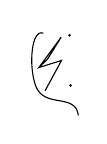
\begin{tikzpicture}[x=.32cm,y=.32cm]
\draw (0.55,2.9) .. controls (0.08,3.1) and (-.05,1.6) .. (.25,.8) .. controls (.6,-.1) and (1.82,.55) .. (1.94,-.36);
\draw (.38,1.55)--(1.26,2.75)--(.72,1.88)--(.37,1.54)--(1.27,1.82)--(.62,.62);
\fill (1.59,2.82) circle (.057) (1.63,.83) circle (.055);
\end{tikzpicture}}

4) \(V'\) \deleted{\unsure{qui est}} en tant que \(\mathbb F_2(\Gamma)\)-module est isom. à \(V\) et irréductible, tandis que \(W\) est une extension non scindée
\diagram{\begin{tikzcd}[ampersand replacement=\&,column sep=small]
0\arrow[r]\&\mathbb F_2\arrow[r,"\lambda\longmapsto\lambda.1"']\&W\arrow[r,"\operatorname{Tr}"']\&\mathbb F_2\arrow[r]\&0
\end{tikzcd}}
\margin{\uline{NB} \(\mathbb F_2.1\) est son propre orthogonal}
\hfill TSVP
